\begin{figure*}
              %\vspace*{-0.25cm}  
        \centering
        \begin{subfigure}[b]{0.35\textwidth}
            \centering
            \caption[]%
            {{Netpipe:64 KB Message}}  
            \vspace*{-0.25cm}  
            \label{fig:jl_netpipe64}
            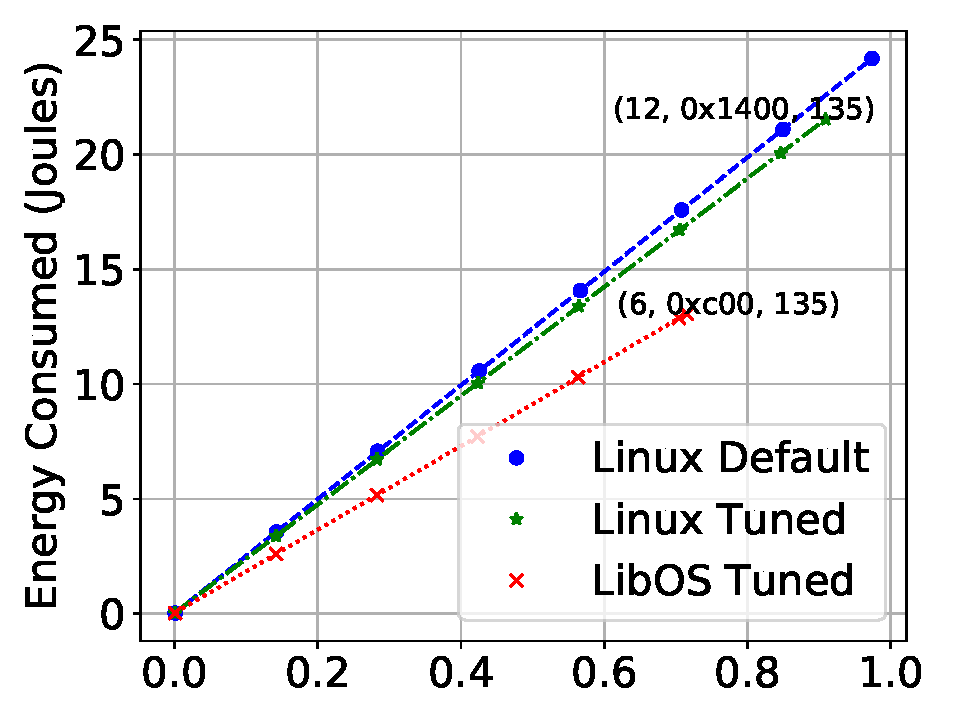
\includegraphics[width=\columnwidth]{osdi_figures/netpipe_65536_epp}
        \end{subfigure}
%        \hfill
        \begin{subfigure}[b]{0.35\textwidth}  
            \centering 
            \caption[]%
            {{Memcached:600K QPS}} 
            \vspace*{-0.25cm}    
            \label{fig:jl_mcd600}
            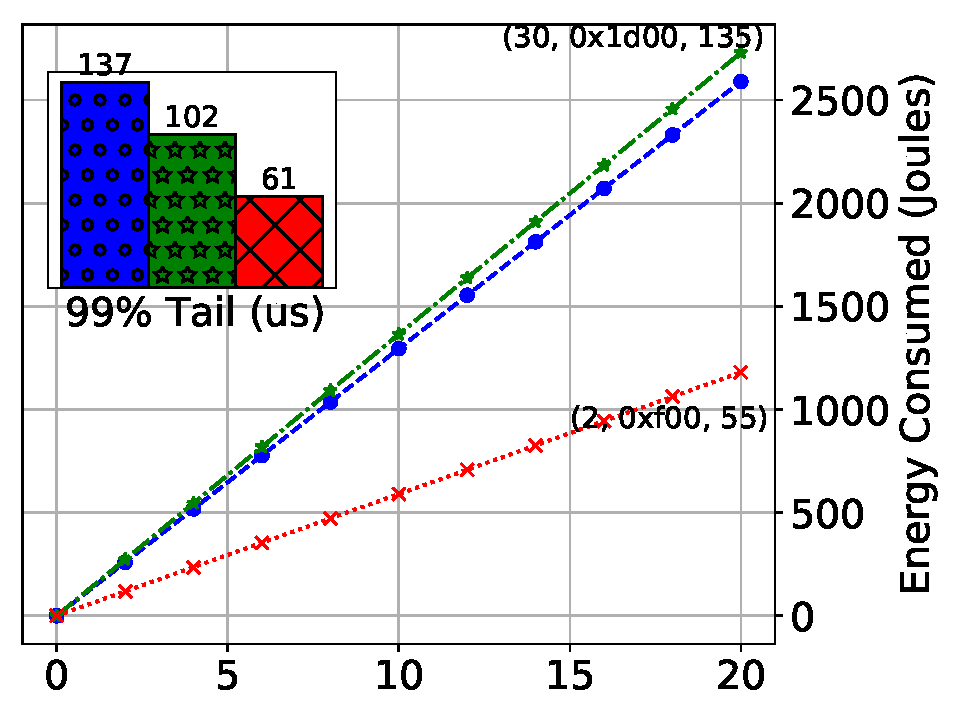
\includegraphics[width=\textwidth]{osdi_figures/mcd_600000_epp}
        \end{subfigure}
        \vskip\baselineskip
        \vspace*{-0.64cm} 
        \begin{subfigure}[b]{0.35\textwidth}   
            \centering 
            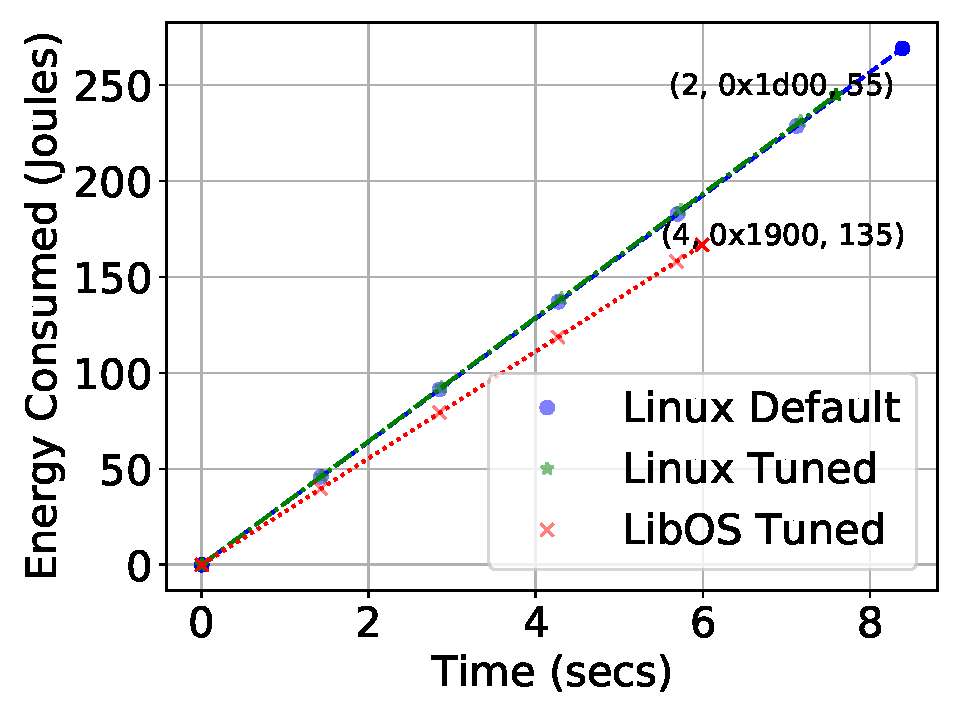
\includegraphics[width=\textwidth]{osdi_figures/nodejs_epp.pdf}
            \caption[]%
                    {{NodeJS}}
                    \vspace*{0.15cm}
            \label{fig:jl_nodejs}
        \end{subfigure}
%        \hfill
        \begin{subfigure}[b]{0.35\textwidth}   
            \centering 
            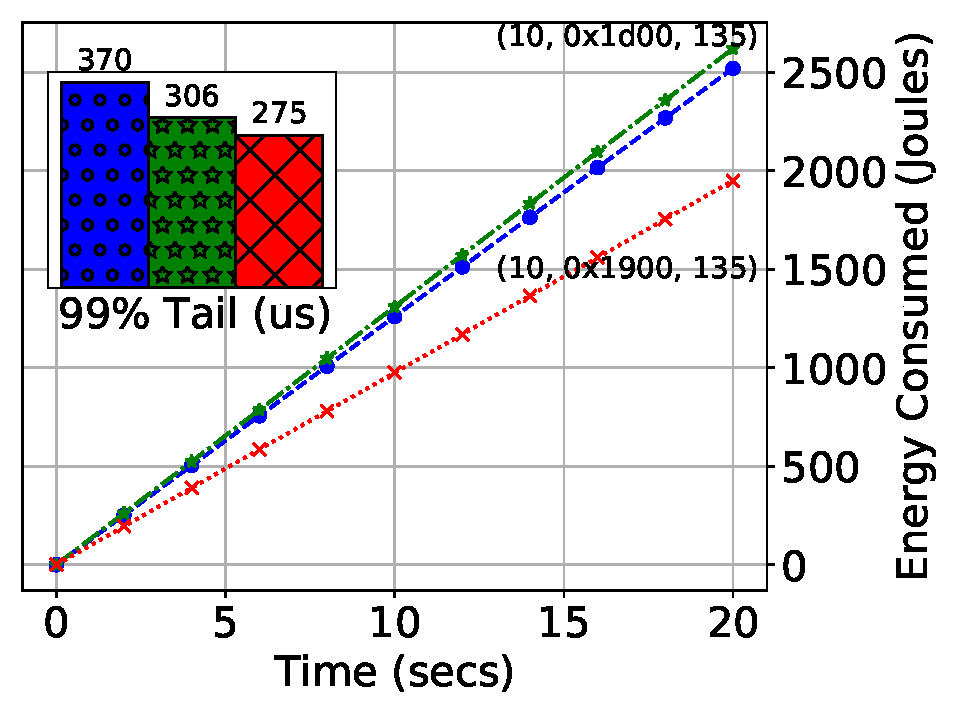
\includegraphics[width=\textwidth]{osdi_figures/mcdsilo_200000_epp}
            \caption[]%
            {{Memcached-silo:200K QPS}}
            \label{fig:jl_mcdsilo200}
        \end{subfigure}
        \caption[]
        {EPP timelines: For each workload we identify the unique hardware settings, for both Linux and libOS, that resulted in the systems best (min) Energy Performance Product (EPP) value. X-axis measures time for each workload (secs), both memcached's ran for 20 secs. The points on each line are a sub-sampling of energy use to improve legibility.
        %Using these values we plot a timeline of the joule readings for one experimental run at the setting for Linux tuned and libOS along with data from a default Linux run of the workload.  The x-axis is the time offset from the beginning of the experiment.  For each log entry with a joule reading, we plot its value against its timestamp offset from the beginning of the run.  While the log has entries for every interrupt, we restrict sampling the joule counter to be at least 1ms apart as per the hardware manual's recommendation, as such not all log entries have an associated joule value.  To improve readability we only show a subset of the markers and use a line to connect the visible marks to the points not shown.    
        } 
        \label{fig:epp}
    \end{figure*}
